\chapter{Background}
\label{chap:background}

%!TEX root = ../main.tex
% \documentclass[float=false, crop=false]{standalone}
% \usepackage[subpreambles=true]{standalone}
% \begin{document}

\section{Background}
\subsection{Augmented Feedback}

\subsection{Pilot Modeling}
\begin{figure}[tb]
    \begin{center}
        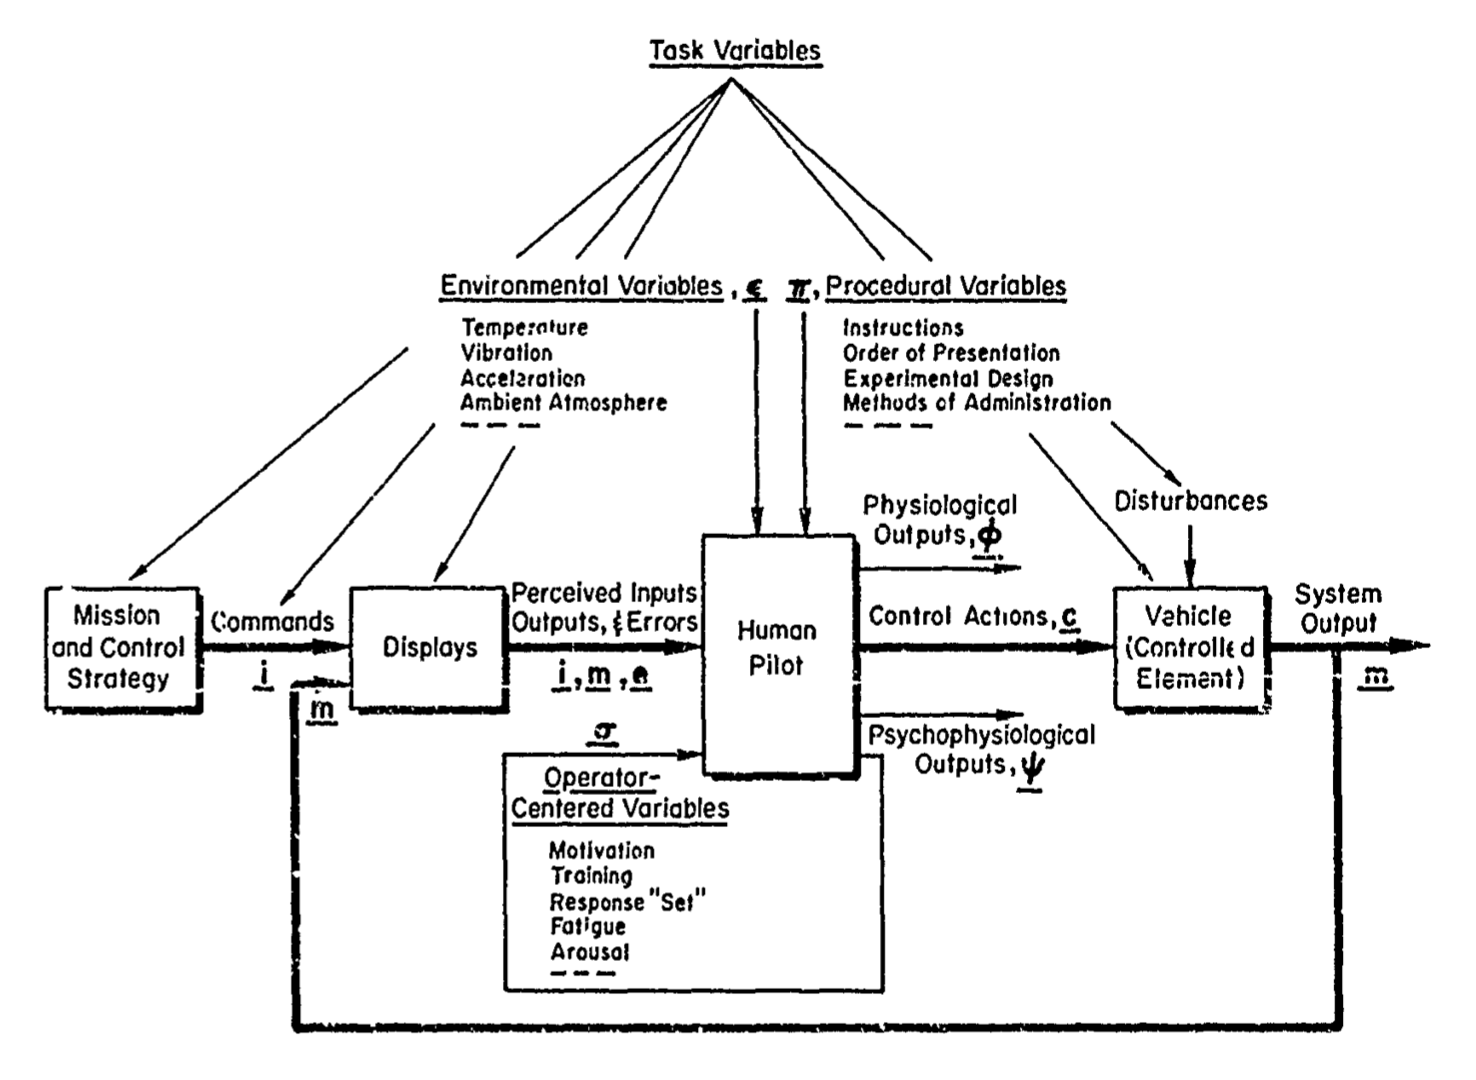
\includegraphics[width=0.8\linewidth]{figures/Screen_Shot_2018-07-25_at_10_37_08_AM.png}
        \caption{Variables affecting the pilot/vehicle system, from~\citep{mcruer_mathematical_1974}.}
        \label{figure:mcruer1974}
    \end{center}
\end{figure}

In addition to popularizing the concept of feedback, the creation of control theory in the early 1940s also provided the tools required for the mathematical modeling of the human pilot.
At the time, new weapons were being created for World War 2 which could only be used effectively with trained operators working in tandem with the machine.
While it was thought that a human could be viewed as a unique kind of servomechanism in the control feedback loop, it was still unclear what factors affected human performance.
Early work by Tustin and others extended the control theory framework and applied these theories to actual human operators~\citep{tustin_investigation_nodate}.
Particular interest was focused on ``attempt[ing] to find the laws of relationship of movement and error. In particular, it was hoped that this relationship [would] be approximately linear and so permit well developed theory of `linear servomechanisms' to be applied to manual control in the same way as it applies to automatic following~\citep{tustin_investigation_nodate}.''
This would allow for the prediction of human performance and the ability to predict the limits of human control.

These early works were summarized in McRuer's 1957 report, ``Dynamic Response of Human Operators''~\citep{mcruer_dynamic_1957}.
This work evaluated measurements for single-input/single-output (SISO) manual control systems and developed predictive models consistent with this data.
Indeed, McRuer writes, ``[i]t is possible, without doing violence to the data, to obtain describing functions which are generally applicable to the results of the many diverse experiments~\citep{mcruer_dynamic_1957}.''
The report concludes by describing a hypothetical transfer function of the human operator which includes a time delay, a neuromuscular lag, and a gain.
McRuer's early model of the complete pilot/vehicle system is presented in Figure~\ref{figure:mcruer1974}.
McRuer revisited these results in 1974, after three decades of supporting engineering and experimental psychology experiments and was able to further generalize these results to a wide variety of system dynamics~\citep{mcruer_mathematical_1974}.
In his study, McRuer completed a detailed analysis which included the human response to proportional, rate/velocity, and acceleration type controlled element dynamics, see Table~\ref{table:mcruer1974a}.
The result of this report was the now famous ``crossover model,'' which relates the operator and controlled element transfer characteristics by the equation
\begin{align}
    Y_c(jw) Y_p(jw) = \dfrac{w_c e^{-jw \tau_e}}{jw}
\end{align}
where $Y_c$ is the controlled element transfer function, $Y_p$ is the approximate human operator transfer function, $w_c$ is the crossover frequency, and $\tau_e$ is the effective time delay of the pilot.
The crossover model is so named as it allows for linear behavior at approximately -20 dB/decade slope in the region of the crossover frequency.
The approximate human operator response to several controlled element transfer functions and their combined open-loop transfer function are presented in Table~\ref{table:mcruer1974b}.
Modeling the human pilot with the crossover enabled a more complete view of the complete pilot/vehicle system, and allowed for human factors recommendations towards the design of new vehicles.
Even today, the crossover model is used as the standard for describing pilot/vehicle systems at the crossover frequency~\citep{mcruer_human_1965, mcruer_mathematical_1974, xu_review_2017}.

\begin{table}[tb]
    \centering
    \caption{Example Applications of Idealized Controlled Element Forms, adapted from~\citep{mcruer_mathematical_1974}}
    \label{table:mcruer1974a}
    \small
    \begin{tabular}{p{.2\linewidth} *{2}{p{.3\linewidth}}}
        \toprule
        Controlled Element Form & Aerospace Control                                & Automobile Control                        \\
        \midrule
        $K_c$                   & Attitude control with ACAH system                & Speed control                             \\
        $\dfrac{K_c}{s}$        & Attitude control with a rate command system      & Heading control at low to moderate speeds \\
        $\dfrac{K_c}{s^2}$      & Attitude control of a spacecraft with damper off & Longitudinal position control             \\
        \bottomrule
    \end{tabular}
\end{table}

\begin{table}[tb]
    \renewcommand{\arraystretch}{2}
    \centering
    \caption{Summary of Human Operator Approximate Characteristics, adapted from~\citep{mcruer_mathematical_1974}}
    \label{table:mcruer1974b}
    \small
    \begin{tabular}{*{3}{c}}
        \toprule
        \thead{Controlled Element                                                            \\ Transfer Function\\ $Y_c$} & \thead{Approximate Human Operator\\ Transfer Function\\ $Y_p$} & \thead{Open-Loop\\ Transfer Function\\ $Y_c Y_p$} \\
        \midrule
        $K_c$              & $\dfrac{K_p e^{-\tau_1 s}}{s}$ & $\dfrac{w_c e^{-\tau_e s}}{s}$ \\
        $\dfrac{K_c}{s}$   & $K_p e^{-\tau_2 s}$            & $\dfrac{w_c e^{-\tau_e s}}{s}$ \\
        $\dfrac{K_c}{s^2}$ & $K_p s e^{-\tau_3 s}$          & $\dfrac{w_c e^{-\tau_e s}}{s}$ \\
        \bottomrule
    \end{tabular}
\end{table}

The continued demand for human pilot models for use in informing vehicle design, as well predicting, preventing, and explaining accidents has led to a variety of more complex pilot models since the creation of the crossover model.
A recent review by Xu et al. in 2017 surveyed the state of the art in human pilot modeling and grouped existing models into three classes of models based on: control theory, human physiology, and intelligence techniques~\citep{xu_review_2017}.
Classical models based on control theory include the McRuer crossover model and optimal control models by Kleinman et al. developed in the early 1970s~\citep{kleinman_optimal_1970, baron_optimal_1970}.
Of these three overarching sets of models, the models based on human physiology are of the greatest interest here.
Models based on human physiology were developed to understand human pilot perception and control behavior, and include the Hess structural model~\citep{hess_structural_1980, hess_model_1990, hess_unified_1997}, Hosman's descriptive model~\citep{hosman_pilots_nodate, hosman_pilots_1999}, and the biodynamic model~\citep{griffin_validation_2001}.
Recent intelligence models take advantage of techniques including fuzzy control and neural networks~\citep{zaychik_conspectus_2006, gestwa_modelling_2003}.

\begin{figure}[tb!]
    \begin{center}
        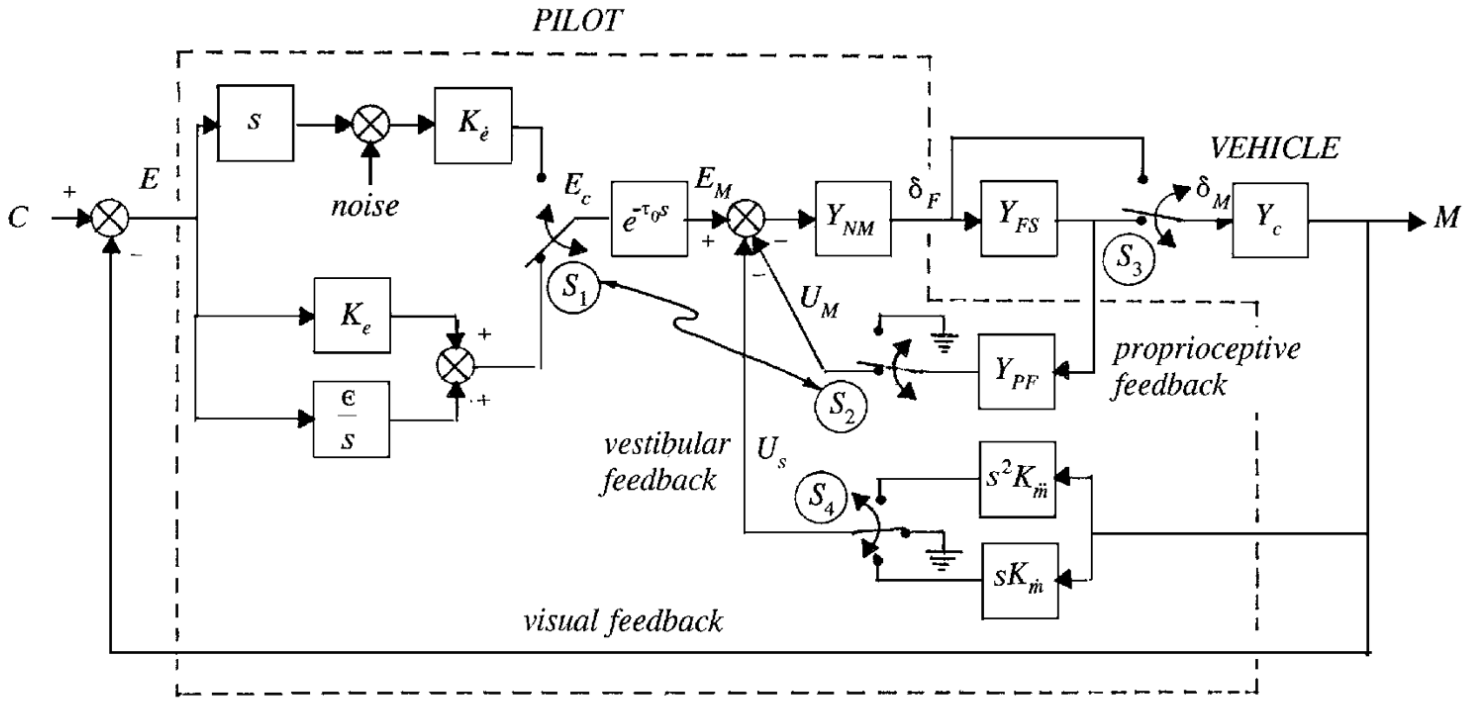
\includegraphics[width=0.8\linewidth]{figures/Screen_Shot_2018-07-31_at_11_21_44_AM.png}
        \caption{The Hess Structural Model of the Human Pilot, from~\citep{hess_unified_1997}.}
        \label{figure:structuralmodel}
    \end{center}
\end{figure}

While the McRuer was very successful in predicting pilot behavior, it it did not attempt ``to describe the underlying structure which contributes to human pilot dynamics~\citep{hess_structural_1980}.''
For this reason, the Hess Structural Model is of particular interest due to the incorporation of multiple sensory channels and models of visual acuity and the time-varying human pilot~\citep{hess_modeling_2009}.
The Structural Model includes the effects of the neuromuscular system, the force-feel characteristics of the input device, and the contributions of proprioceptive, vestibular, and visual feedback, see Figure~\ref{figure:structuralmodel}.
One of the key strengths of the Structural Model is the relatively few number of free parameters that need to be set to predict pilot performance.
The model has been used in predicting and evaluating handling qualities and pilot-induced oscillation rating levels for helicopters, Boeing 747, Lockheed C-5A, and twin ducted-fan aircraft~\citep{hess_analytical_2013, andreea-irina_prediction_2014, grant_handling_2015}.
Hess has also investigated how pilot control characteristics change with time due to flight anomalies, changing flight dynamics, and sudden increases in task demand~\citep{hess_modeling_2009, hess_modeling_2016}.
The results of this model have been compared to the results of a human-in-the-loop simulation for a well trained subject, and showed good comparison~\citep{hess_modeling_2016}.
Recent work from Bachelder et al. has included modifications to the Structural Model to link pilot performance and workload and to enable the modeling of pulsive pilot behavior~\citep{bachelder_modeling_2017, bachelder_linking_2018}.

%!TEX root = ../main.tex
% \documentclass[float=false, crop=false]{standalone}
% \usepackage[subpreambles=true]{standalone}

% \begin{document}
\section{Problem Statement}
\subsection{Motivation}
We aim to improve performance and decrease learning times for novice operators of highly complex motor control tasks.
We are specifically interested in modeling and improving human performance in robotic arm tasks, which generally require extensive training to master.
The robotic arm on the International Space Station (ISS), for instance, requires hundreds of hours of training time for astronauts to reach proficiency.
Being able to decrease this training time could lead to significant savings in cost, and the predictive ability provided by modeling human performance allows for safer operation of the robotic arm.

A variety of skills can be classified as motor control tasks, such as playing tuba, pole vaulting, or flying an aircraft.
An individual's performance in any of these skills can change dramatically as they transition from a novice to an expert through training.
We are interested in measuring and modeling this performance as it changes over the course of the training process.

Humans rely on several kinds of feedback during training to improve their performance in motor control tasks.
Feedback can be largely grouped into two types: internal, or intrinsic feedback, and external, or extrinsic feedback.
Intrinsic feedback is anything a person can infer using their senses: the feel of the valves of the tuba as you play, the sense of balance mid-jump, or the sound the aircraft engine makes during a climb.
Extrinsic feedback, conversely, is provided by an external source, often in the form of an expert instructor.
Extrinsic feedback comes in a variety of forms, and has a long history of improving performance in a large variety of motor control tasks.

We will focus on a specific type of extrinsic feedback, which is known as concurrent bandwidth feedback (CBF).
Concurrent feedback is provided in real-time, as an operator is completing a task.
Bandwidth feedback is provided when a objective particular value deviates outside a designated range or bandwidth.
Concurrent bandwidth feedback is, therefore, feedback provided to an operator in real-time when a signal deviates out of a predefined range.
This type of feedback has been shown to improve performance in many simple motor control tasks, but has not been investigated in complex, high degree of freedom tasks.

It is important to note that this feedback should be thought of as qualitative feedback, not as an additional form of quantitative guidance.
We are not interested in adding additional displays or gauges to control interfaces, but would prefer to modify existing indicators, during training, to better inform an operator as to how well they are performing a task.
Despite extensive evidence as to the effectiveness of this feedback, the mechanism by which performance is improved has yet to be explained, nor integrated into human performance models.
We will attempt to explain why this feedback is effective in enhancing learning and integrate this explanation into a model.

\subsection{Research Aims}
We are interested in measuring, modeling, and predicting the effects of concurrent bandwidth feedback (CBF) on human performance in robotics manual control tasks.
To this end, this proposed research includes three research aims.
These aims build on each other, starting with a compensatory tracking task, extending to a robotics task, and finishing with a descriptive model describing both.
The first aim is complete, and the second and third aims are in progress.
\begin{description}[align=left]
    \item [Aim One] Investigate the effects of concurrent bandwidth feedback on human performance and workload effects in a three-axis manual tracking task.
    \item [Aim Two] Investigate the effects of concurrent bandwidth feedback on human performance and workload effects in a robotics track and capture task.
    \item [Aim Three] Extend the Hess Structural Model of the human pilot to include the effects of concurrent bandwidth feedback.
\end{description}

There are a number of research questions that we intend to answer by completing these aims, which include:
\begin{enumerate}
    \item Can concurrent bandwidth feedback improve human performance in a three-axis manual tracking task?
          \begin{enumerate}
              \item Do 3D augmented reality displays show improved performance compared to traditional 2D displays?
              \item Can performance be increased without increasing workload?
          \end{enumerate}
    \item Can concurrent bandwidth feedback improve performance of simulated robotics tasks?
          \begin{enumerate}
              \item Can CBF reduce the required training time to peak performance?
              \item Can CBF be removed after reaching peak performance without reducing subject performance?
              \item Can performance be increased without increasing workload?
          \end{enumerate}
    \item Can we develop a descriptive model of human performance which includes the effects of concurrent bandwidth feedback?
          \begin{enumerate}
              \item Can we use this model to estimate operational limits?
          \end{enumerate}
\end{enumerate}

The remainder of this proposal is divided into three sections: a literature review, the proposed research, and a timeline.

%!TEX root = ../main.tex
% \documentclass[float=false, crop=false]{standalone}
% \usepackage[subpreambles=true]{standalone}

% \begin{document}

\section{Proposed Research}
We propose to run human-in-the-loop subject testing experiments to understand the effects of concurrent bandwidth feedback, and to integrate the effects of this feedback into a human performance model.
To investigate the three Aims outlined in the Problem Statement, we propose two experiments and the development of a model.

\begin{description}[align=left]
    \item [Experiment One] investigates if concurrent bandwidth feedback can be used to teach novice subjects to improve performance in a three-axis manual tracking task.
    \item [Experiment Two] investigates if concurrent bandwidth feedback can decrease the required learning time to peak performance in a simulated robotic arm track and capture task.
    \item [The Model] will extend Professor Hess' structural model of the human pilot to include the effects of concurrent bandwidth feedback.
\end{description}

Concurrent bandwidth feedback has been used in a large variety of motor control tasks, and has generally been found to improve performance.
Until recently, however, only simple tasks such as physical movements or low-dimensional pursuit tasks have been investigated.
More recent works, including the lane-keeping task by de Groot et al., and our previous work with the SAFER task, have indicated that concurrent bandwidth feedback can also be quite effective for complex tasks.
Unlike simple tasks, in which the guidance hypothesis dominates when feedback is removed, there is some evidence that concurrent bandwidth feedback can be removed after training without a loss of performance.
The decrease in required learning time, improved performance, and decreased workload seen in the SAFER task show that concurrent bandwidth feedback may prove to be most useful very early in training when subjects are first exposed to complex, highly dynamic tasks.
As concurrent bandwidth feedback can improve performance without an increase in workload, it may prove a useful technique for training other robotics tasks.

There has been considerable improvement in the field of pilot modeling since McRuer's crossover model, especially with models that incorporate human physiology.
The Structural Model, in particular, has been very effective in predicting pilot performance, handling qualities, pilot-induced oscillation rating levels, and workload for a variety of system dynamics.
None of these pilot models, however, are able to include the effects of concurrent bandwidth feedback.
The performance improving effects of this feedback, seen throughout the literature, make this a compelling feature to be incorporated into a pilot model.

\subsection{Experiment Two}
\begin{figure}[tb]
    \begin{center}
        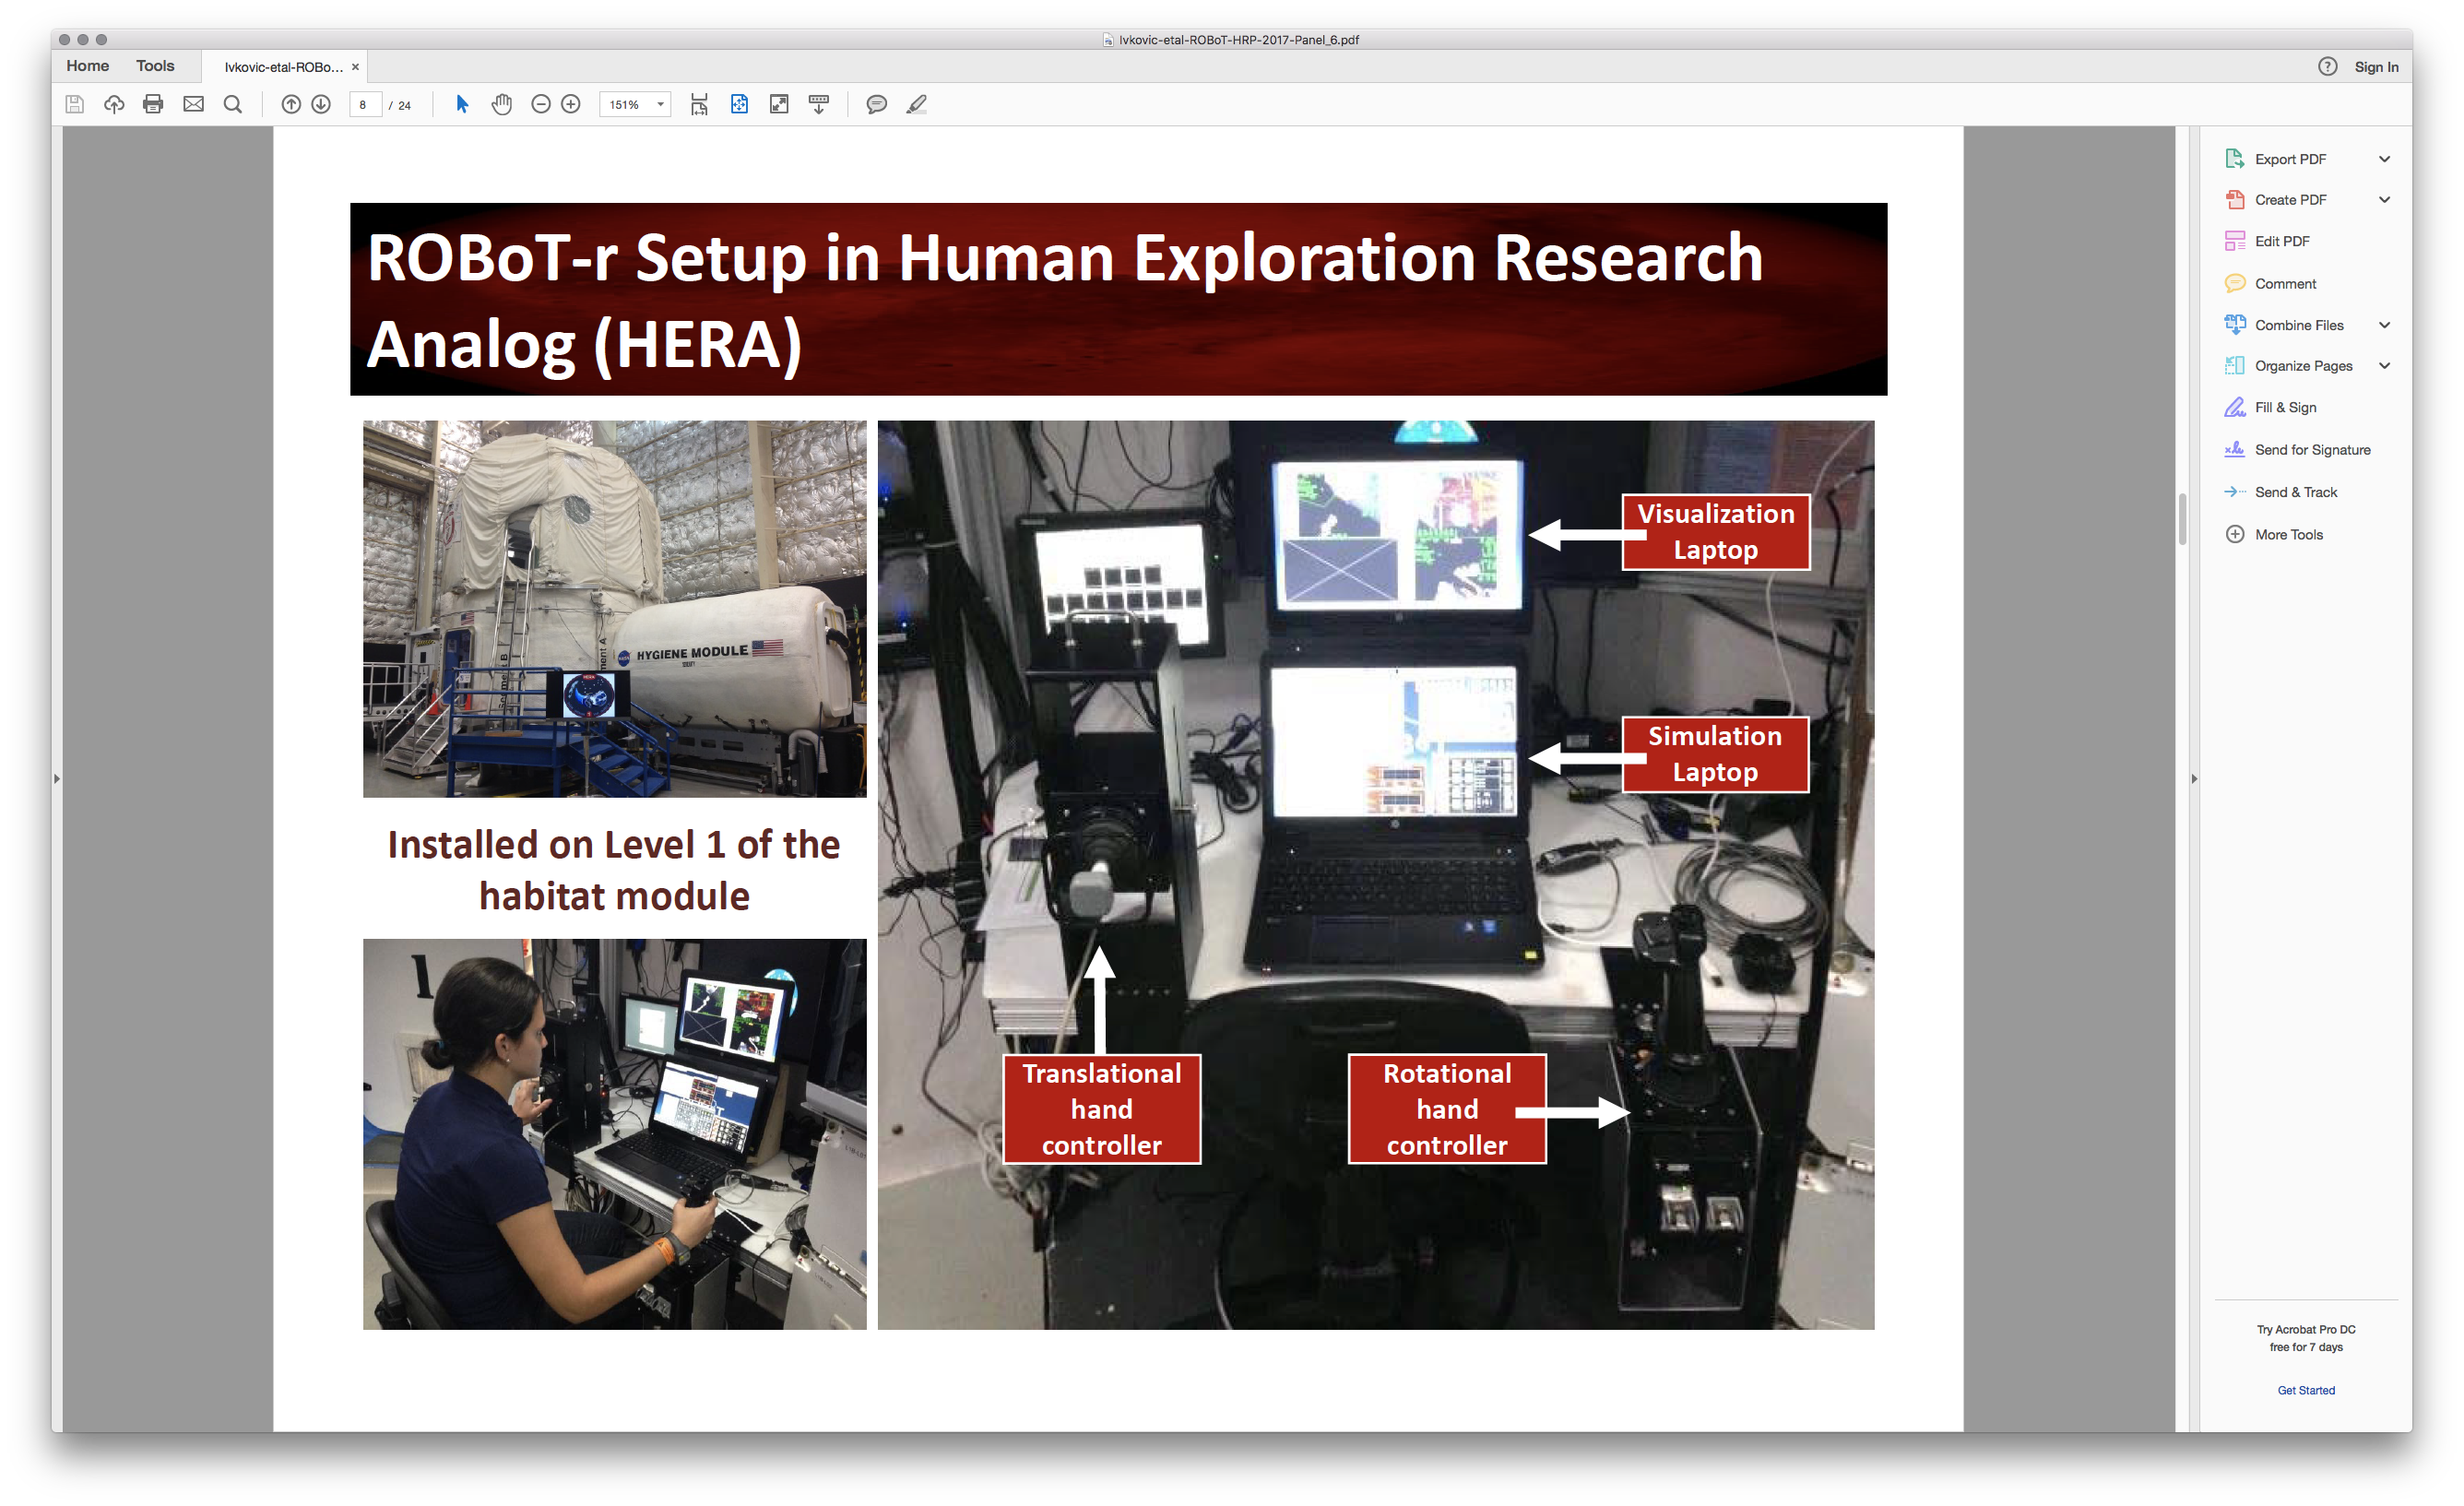
\includegraphics[trim={13cm 5cm 22cm 15.5cm},clip,width=\linewidth]{figures/Screen_Shot_2018-07-26_at_1_43_16_PM.png}
        \caption{The Robotic On-board Trainer (ROBoT) station set up in the NASA HERA Analog, from~\citep{robottalk}.}
        \label{figure:robotinhera}
    \end{center}
\end{figure}

The second Aim of the proposal is addressed by Experiment Two.
Experiment Two will focus on if concurrent bandwidth feedback can decrease the required learning time to peak performance in a simulated robotic arm track and capture task.
We will compare task performance throughout training and workload between two groups: a control group, which receives no feedback, and a treatment group, which receives concurrent bandwidth feedback on one or more sensor readouts.
Subjects in both groups will complete the same task, and it is hypothesized that subjects in the treatment group will perform the task better and require less training time to reach peak performance.
This hypothesis is based on the results of the SAFER experiment, as well as the results of Experiment One.

In this task, subjects will command a robotic arm to track an approaching vehicle and grapple with it.
This is motivated by the primary use of the robot arm on the International Space Station, which grasps visiting vehicles when they arrive at the station and then attaches them to a separate fixed location on the station.
Subjects will be trained on this task and will then repeat the task for one to two hours through a variety of slightly different start and end conditions.

NASA's Robotic On-board Trainer (ROBoT) will be used for this experiment.
ROBoT is a package of simulation software which includes a dynamic model of the robotic arm on the space station and presents the user with multiple camera angle views and the instrument panel required to operate the robotic arm, see Figure~\ref{figure:robotinhera}.
In addition to these displays, ROBoT also includes the two hand controllers required to control the arm.
NASA trainers at Johnson Space Center developed metrics for performance which are included in ROBoT and include the time to capture, the alignment measurements during approach, the amount of wobble in the arm, the number of times the grapple fixture contacted the structure, the overall path efficiency, and the number of capture attempts.
The preceding list presents candidate metrics from which we may observe human performance.

\subsubsection{Hypotheses}
This study will assess the influence of concurrent bandwidth feedback (with vs. without) on performance and workload.
Objective performance data will be measured using time to capture, alignment error metrics, and other metrics available by the ROBoT system.
Subjective workload will be measured using the NASA-TLX at several points throughout the experiment.
It is hypothesized that:
\begin{description}[align=left]
    \item [Hypothesis 1] Concurrent bandwidth feedback will improve performance in the track-and-capture task.
    \item [Hypothesis 2] Concurrent bandwidth feedback will cause subjects to more quickly reach their peak performance in the track-and-capture task.
    \item [Hypothesis 3] Concurrent bandwidth feedback will decrease workload in the track-and-capture task.
\end{description}

\subsubsection{Previous Work}
We have experience using the ROBoT simulation software from participating in a study investigating the effects of sleep loss and circadian misalignment on performance on the ROBoT simulator at NASA Ames~\citep{robotreport}.
In this study, subjects trained during one-hour long sessions each day for five days, then spent a twenty four hour period in the lab while they continued to perform robotic tasks.
We did not find evidence of performance loss during sleep deprivation or circadian misalignment on any of the ROBoT performance metrics.
In fact, participants continued to show improvement over time, which indicated that they had continued to learn the task despite the sleep loss~\citep{robotreport}.
This finding reinforces the need for enhanced learning techniques, as the current training strategy requires a tremendous amount of time to reach peak performance.

% \begin{figure}[tb!]
%     \begin{center}
%         \includegraphics[trim={13cm 5cm 22cm 15.5cm},clip,width=\linewidth]{./../img/Screen Shot 2018-07-26 at 1.43.02 PM.png}
%         \caption{ROBoT visualization laptop, showing four camera views.}
%         % \label{}
%     \end{center}
% \end{figure}

% \begin{figure}[tb!]
%     \begin{center}
%         \includegraphics[trim={13cm 5cm 22cm 15.5cm},clip,width=\linewidth]{./../img/Screen Shot 2018-07-26 at 1.43.05 PM.png}
%         \caption{The camera attached to the end effector of the robotic arm, showing the grapple fixture.}
%         % \label{}
%     \end{center}
% \end{figure}

% \begin{figure}[tb!]
%     \begin{center}
%         \includegraphics[trim={13cm 5cm 22cm 15.5cm},clip,width=\linewidth]{./../img/Screen Shot 2018-07-26 at 1.43.07 PM.png}
%         \caption{Example performance score report shown to the user after each trial.}
%         % \label{}
%     \end{center}
% \end{figure}

% \begin{figure}[tb!]
%     \begin{center}
%         \includegraphics[trim={13cm 5cm 22cm 15.5cm},clip,width=\linewidth]{./../img/Screen Shot 2018-07-26 at 1.43.10 PM.png}
%         \caption{The hand controller inputs and position and angular errors are also logged throughout the trial.}
%         % \label{}
%     \end{center}
% \end{figure}

\subsection{Model Extension}
The third and final Aim of the proposal is addressed by developing a model of the human pilot which includes the effects of concurrent bandwidth feedback.
The proposed Model will extend Professor Hess' structural model of the human pilot to include the effects of concurrent bandwidth feedback.
The Structural Model has been extremely successful in predicting human performance through a variety of system dynamics and can predict how performance changes during a pilot's adaptation to changing dynamics.
Hess has developed adaptive logic for the human pilot in a pursuit task which triggers when the pilot notices that vehicle dynamics have changed~\citep{hess_modeling_2009}.
This logic is based off several criteria, which ``must be predicated upon information available to the human [and] the postadapated pilot models must follow the dictates of the crossover model of the human pilot~\citep{hess_modeling_2009}.''
The primary result of the adaptive logic is to increase the resulting crossover frequency of the pilot, effectively making them more responsive, which could be interpreted as more focused on the task.
Our initial approach to adding concurrent bandwidth feedback into the Structural Model will be based off of Hess' approach to modeling human adaptation in pursuit tasks, which is currently ad-hoc in nature, see Figure~\ref{figure:hesspursuit}.

\begin{figure}[tb]
    \begin{center}
        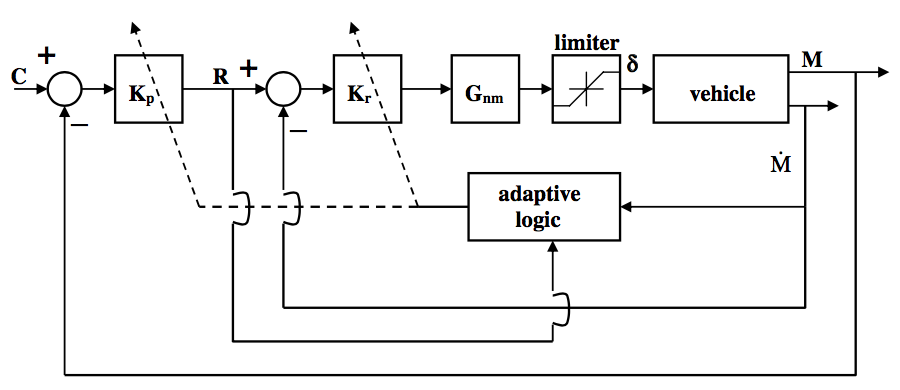
\includegraphics[width=0.8\linewidth]{figures/Screen_Shot_2018-08-09_at_4_15_24_PM.png}
        \caption{Hess' model of the adaptive human pilot, from~\citep{hess_modeling_2009}.}
        \label{figure:hesspursuit}
    \end{center}
\end{figure}

While this model of the adaptive pilot has been successful in predicting changes in performance for a well trained subject, it does not consider how a pilot would behave when they are still in the early stages of training.
Our modified model will include two major changes to Hess' current model:
\begin{itemize}
    \item The adaptation logic will be changed to focus on concurrent bandwidth feedback
    \item The timescale of the adaptation will be significantly longer
\end{itemize}

We propose to modify the adaptive logic to trigger when the pilot is receiving concurrent bandwidth feedback, rather than when a change in system dynamics occurs.
This will require the addition of a feedback loop onto the Structural Model which triggers when the bandwidth feedback is activated.
This loop will likely be based around the $K_e$ gain, which is currently the primary way of setting the crossover frequency in the Structural Model.
This implies that the subjects in our experiments do their primary learning when they are receiving qualitative feedback that their current level of aggressiveness is not sufficient to complete the task.
While there must be a separate loop that adjusts the crossover frequency as learning progresses over the course of several hours, the change in performance we see when subjects use the concurrent bandwidth feedback happens relatively rapidly, within a few minutes.
This is reflected in the delta of performance between subjects in the different groups of our SAFER experiment, even on the first trial, see Figure~\ref{figure:saferdistance}.
This relates to the second required change, the amount of required adaptation time.
Professor Hess' model requires that pilots adapt within a very short time period, on the order of 5 seconds~\citep{weir_model_1966}.
The results of our experiment with SAFER and the three-axis tracking task also suggest relatively short adaptation times, though they are on the order of a few minutes, again see Figure~\ref{figure:saferdistance}.

While it should be noted that this work is in preliminary stages and not scheduled to begin until the Fall Quarter, some early work has been started in preparation for the qualifying examination.
An effort has been made to begin to replicate some of Hess' results.
Working with Professor Hess, we have been able to replicate some of the existing adaptation logic for a two-axis tracking task, and begun exploratory research into modifying the model.

%!TEX root = ../main.tex
% \documentclass[float=false, crop=false]{standalone}
% \usepackage[subpreambles=true]{standalone}
% \begin{document}

\section{Timeline and Risks}
% \begin{figure}[h!]
%     \begin{center}
%         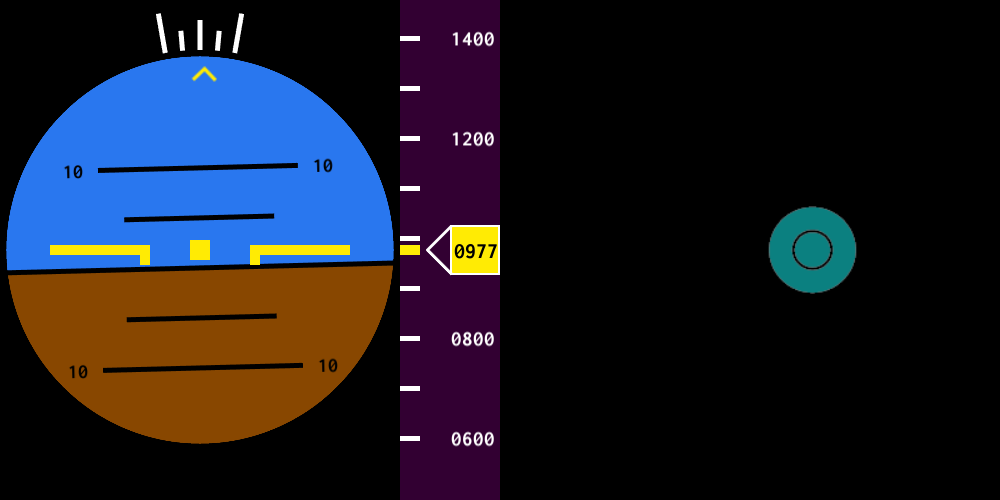
\includegraphics[width=\linewidth]{./../img/image1.png}
%         \caption{The proposed timeline for this research.}
%         \label{timeline}
%     \end{center}
% \end{figure}

The proposed timeline for the remainder of this research is available in Figure%~\ref{timeline}.
This timeline shows the past few months spent accomplishing the first aim and outlines our estimated timeline to complete the remaining aims, with an estimated graduation date of Summer Quarter 2020.
While not present on the timeline, we also plan to write and submit several conference papers and journal articles throughout the completion of this research.

A conference paper, ``Evaluating Augmented Reality in a Three-Axis Manual Tracking Task'', J. Karasinski and S. Robinson has recently been submitted for consideration at AIAA SciTech 2018.
A draft journal article on the SAFER experiment is being prepared for submission in the journal of Human Factors.
We expect to publish an additional conference paper to an AIAA or IEEE conference and journal article for the results of the robotic arm experiment, likely in Human Factors.
If we are successful in creating a model which closely follows human behavior, we would also publish this as a journal article, likely in the Journal of Guidance, Control, and Dynamics.

% This timeline was created under the assumption that everything will go according to plan, which is almost certainly not the case.
This schedule is flexible to changes in plans, and was designed with the full awareness that we may face setbacks.
There are a number of places where we may suffer delays or other issues:
\begin{itemize}
    \item% 
          % It is difficult to predict how long it will take to recruit subjects and run them through an experiment.
          While the author has experience subject testing over one hundred subjects over three hundred hours of experiment time, it is difficult to predict how long subject testing will take to complete.
          Under the assumption that we will run approximately twenty to thirty subjects in the robotic arm experiment, and that the experiment will last for approximately two to three hours per subject, we have budgeted one quarter to recruit subjects and run them through the experiment.
          This could, however, easily stretch to two quarters, depending on subject availability and success rates.
    \item NASA Ames has agreed to allow the Human/Robotics/Vehicle Integration and Robotics Lab to use the ROBoT simulator for this proposed experiment at UC Davis.
          If, for whatever reason, we are unable to use ROBoT, we could either run the experiment at Ames or attempt to build our own robotic arm simulation.
    \item While we believe we have sufficient evidence that our feedback techniques will improve performance, it is also possible that we will not see significant effects in the robotic arm task.
          If this is the case we will need to further investigate how this task is different from our previous successes.
          This would allow us, for instance, to make begin to make recommendations for which types of tasks can and cannot benefit from this feedback.
    \item It is possible that we may be unable to create a model which incorporates feedback and that accurately mirrors the effects we have seen in our experiments. This may require us to investigate other types of performance models or to create a novel technique.
\end{itemize}
